\documentclass[technicalreport]{ieicej}
\usepackage[dvipdfmx]{graphicx}
\usepackage[T1]{fontenc}
\usepackage{lmodern}
\usepackage{textcomp}
\usepackage{latexsym}
\usepackage{amsmath}
\usepackage{cite}
\usepackage{tikz}
\usepackage{geometry}
\usepackage{url}
\usepackage{schemabloc}
\usepackage{tikz}
\usetikzlibrary{arrows}

\usetikzlibrary{positioning,fit,calc}
\tikzset{block/.style={draw, thick, text width=1cm, minimum height=0.5cm, align=center}, line/.style={-latex}}  

\renewcommand{\figurename}{Fig.} % name the picture Fig.num
\renewcommand{\tablename}{Table } % name the table Table num
\renewcommand{\refname}{REFERENCE} % insert reference 

%调整文件显示位置和纸张
\geometry{
	a4paper,
	total={170mm,257mm},
	left=20mm,
	top=20mm,
}

\hoffset=-5mm
\voffset=-5mm

\def\IEICEJcls{\texttt{ieicej.cls}}
\def\IEICEJver{3.0}
\newcommand{\AmSLaTeX}{%
$\mathcal A$\lower.4ex\hbox{$\!\mathcal M\!$}$\mathcal S$-\LaTeX}
\def\BibTeX{{\rmfamily B\kern-.05em{\scshape i\kern-.025em b}\kern-.08em
T\kern-.1667em\lower.7ex\hbox{E}\kern-.125em X}}

\jtitle{M1課題レポート 第2回目}
\jsubtitle{}
\etitle{Technical Report for M1 Labwork 2nd}
\esubtitle{}
\authorlist{
\authorentry[liuyuchen@radio.ict.e.titech.ac.jp]{りゅう ゆしん}{Yuchen Liu}{Titech}
}

\affiliate[Titech]{東京工業大学 〒152-8550 東京都目黒区大岡山2-12-1}
{Tokyo Institute of Technology,~~2-12-1, O-okayama, Meguro-ku, Tokyo, 152-8550 Japan}

\begin{document}

\begin{eabstract}

\end{eabstract}

\maketitle

\section{Introduction}


\begin{table}[tbp]
	\begin{center}
	\caption{MAPPING TABLE OF PHASE}
	\begin{tabular}{ll}
	\hline
	\textbf{bitA bitB} & \textbf{$\Delta\theta_{i}$} \\
	\hline
	0 0 & $0$ \\
	1 0 & $\frac{pi}{2}$ \\
	1 1 & $\pi$ \\
	1 0 & $\frac{3\pi}{2}$ \\
	\hline
	\end{tabular}
	\end{center}
\end{table}

\begin{table}[hb]
	\begin{center}
	\caption{SIMULATION CONDITIONS}
	\label{tbl:simu}
	\small
	\begin{tabular}{ll}
	\hline
	ITEMS & CONDITIONS\\
	\hline
	Moduation Method & DQPSK \\
	Transmission Bits & 128 \\
	Channel & AWGN \\
	Detection & Noncoherent and Coherent Detection \\
	Number of Trials & $10^{6}$\\
	Distribution of Phase Shift & $U[0,2\pi]$\\
	\hline
	\end{tabular}
	\end{center}
\end{table}

\section{Simulation and Result}


\begin{figure}[tbp]
	\begin{center}
		\vspace{0cm}
		\includegraphics[width=\linewidth,clip]{fig/without_shift.eps}
		\caption{Coherent Reception and Non-coherent Reception Without Phase Shift}
		\label{fig:sample}
	\end{center}
\end{figure}

\begin{figure}[tbp]
	\begin{center}
		\vspace{0cm}
		\includegraphics[width=\linewidth,clip]{fig/phase_shift.eps}
		\caption{Coherent Reception and Non-coherent Reception With Phase Shift}
		\label{fig:sample}
	\end{center}
\end{figure}

\section{Conclusion}


\bibliographystyle{IEEEtran}
\bibliography{non_coherent.bib}

\end{document} 